\documentclass[12pt,twoside]{mitthesis}
%\usepackage{lgrind}

\usepackage[square,comma,numbers,sort&compress]{natbib}
\usepackage{amsmath,amsthm,amssymb,amsfonts,amsbsy,latexsym}
\usepackage{graphics}
\usepackage{epsfig}
%\usepackage[hang,raggedright]{subfigure}
\usepackage{epsf}
\usepackage{setspace}
\usepackage{hangcaption}
\usepackage{graphicx}    % needed for including graphics e.g. EPS, PS
\usepackage{multirow}
\usepackage{threeparttable}
\usepackage{cancel}
\usepackage{enumerate}
\usepackage{color}
\usepackage{hyperref}

\usepackage{algorithmicx}
\usepackage[ruled]{algorithm}
\usepackage{algpseudocode}
\usepackage{varwidth}
\usepackage{caption}
\usepackage[font=small]{subcaption}
\usepackage{longtable}
\usepackage{mathrsfs}

\hypersetup{
    colorlinks=true,       % false: boxed links; true: colored links
    linkcolor=black,          % color of internal links
    citecolor=black,        % color of links to bibliography
    filecolor=magenta,      % color of file links
    urlcolor=blue           % color of external links
}

\newcommand{\R}{{\mathbb{R}}}
\newcommand{\bit}{\begin{itemize}}
\newcommand{\eit}{\end{itemize}}
\newcommand{\red}[1]{{\color{red}{#1}}}

\graphicspath{{./figures/}}

\begin{document}
\raggedbottom %avoid weird vertical justification

%!TEX root = ../main_v01.tex

\title{Model Adaptivity for Goal-Oriented Inference}
%\fontsize{15}{17}\selectfont 
\author{Harriet Li}

\prevdegrees{B.S. Aerospace Engineering (2013)\\
             Massachusetts Institute of Technology}

\department{Department of Aeronautics and Astronautics}
% If the thesis is for two degrees simultaneously, list them both
% separated by \and like this:
% \degree{Doctor of Philosophy \and Master of Science}
\degree{Master of Science}
\degreemonth{June}
\degreeyear{2015}
\thesisdate{May 21, 2015}

%% By default, the thesis will be copyrighted to MIT.  If you need to copyright
%% the thesis to yourself, just specify the `vi' documentclass option.  If for
%% some reason you want to exactly specify the copyright notice text, you can
%% use the \copyrightnoticetext command.  
%\copyrightnoticetext{\copyright IBM, 1990.  Do not open till Xmas.}

% If there is more than one supervisor, use the \supervisor command
% once for each.
\supervisor{Karen Willcox}{Professor of Aeronautics and Astronautics}

% This is the department committee chairman, not the thesis committee
% chairman.  You should replace this with your Department's Committee
% Chairman.
\chairman{Paulo Lozano}{Associate Professor of Aeronautics and Astronautics\\
        Chair, Graduate Student Committee}


% Make the titlepage based on the above information.  If you need
% something special and can't use the standard form, you can specify
% the exact text of the titlepage yourself.  Put it in a titlepage
% environment and leave blank lines where you want vertical space.
% The spaces will be adjusted to fill the entire page.  The dotted
% lines for the signatures are made with the \signature command.
\maketitle

% The abstractpage environment sets up everything on the page except
% the text itself.  The title and other header material are put at the
% top of the page, and the supervisors are listed at the bottom.  A
% new page is begun both before and after.  Of course, an abstract may
% be more than one page itself.  If you need more control over the
% format of the page, you can use the abstract environment, which puts
% the word "Abstract" at the beginning and single spaces its text.

%% You can either \input (*not* \include) your abstract file, or you can put
%% the text of the abstract directly between the \begin{abstractpage} and
%% \end{abstractpage} commands.

% First copy: start a new page, and save the page number.
\cleardoublepage
% Uncomment the next line if you do NOT want a page number on your
% abstract and acknowledgments pages.
% \pagestyle{empty}
\setcounter{savepage}{\thepage}

%Uncomment the following three lines if you want an abstract page
\begin{abstractpage}
In scientific and engineering contexts, physical systems are represented by mathematical models, characterized by a set of parameters. The inverse problem arises when the parameters are unknown and one tries to infer these parameters based on observations. Solving the inverse problem can require many model simulations, which may be expensive for complex models; multiple models of varying fidelity and complexity may be available to describe the physical system. However, inferring the parameters may only be an intermediate step, and what is ultimately desired may be a low-dimensional Quantity of Interest (QoI); we refer to this as the goal-oriented inverse problem. We present a novel algorithm for solving the goal-oriented inverse problem, which allows one to manage the fidelity of modeling choices while solving the inverse problem.

We formulate a hierarchy of models, and assume that the QoI obtained by inferring the parameters with the highest-fidelity model is the most accurate QoI. We derive an estimate for the error in the QoI from inferring the parameters using a lower-fidelity model instead of the highest-fidelity model. This estimate can be localized to individual elements of a discretized domain, and this element-wise decomposition can then be used to adaptively form mixed-fidelity models. These mixed-fidelity models can be used to infer the parameters, while controlling the error in the QoI.

We demonstrate the method with two pairs of steady-state models in 2D. In one pair, the models differ in the physics included; in the other pair, the models differ in the space to which the parameters belong. In both cases, we are able to obtain a QoI estimate with a small relative error without having to solve the inverse problem with the high-fidelity model. We also demonstrate a case where solving the inverse problem with the high-fidelity model requires a more complex algorithm, but where our method gives a mixed-fidelity model with which we can infer parameters using a simple Newton solver, while achieving a low error in the QoI.


\end{abstractpage}

% Additional copy: start a new page, and reset the page number.  This way,
% the second copy of the abstract is not counted as separate pages.
% Uncomment the next 6 lines if you need two copies of the abstract
% page.
% \setcounter{page}{\thesavepage}
% \begin{abstractpage}
% In scientific and engineering contexts, physical systems are represented by mathematical models, characterized by a set of parameters. The inverse problem arises when the parameters are unknown and one tries to infer these parameters based on observations. Solving the inverse problem can require many model simulations, which may be expensive for complex models; multiple models of varying fidelity and complexity may be available to describe the physical system. However, inferring the parameters may only be an intermediate step, and what is ultimately desired may be a low-dimensional Quantity of Interest (QoI); we refer to this as the goal-oriented inverse problem. We present a novel algorithm for solving the goal-oriented inverse problem, which allows one to manage the fidelity of modeling choices while solving the inverse problem.

We formulate a hierarchy of models, and assume that the QoI obtained by inferring the parameters with the highest-fidelity model is the most accurate QoI. We derive an estimate for the error in the QoI from inferring the parameters using a lower-fidelity model instead of the highest-fidelity model. This estimate can be localized to individual elements of a discretized domain, and this element-wise decomposition can then be used to adaptively form mixed-fidelity models. These mixed-fidelity models can be used to infer the parameters, while controlling the error in the QoI.

We demonstrate the method with two pairs of steady-state models in 2D. In one pair, the models differ in the physics included; in the other pair, the models differ in the space to which the parameters belong. In both cases, we are able to obtain a QoI estimate with a small relative error without having to solve the inverse problem with the high-fidelity model. We also demonstrate a case where solving the inverse problem with the high-fidelity model requires a more complex algorithm, but where our method gives a mixed-fidelity model with which we can infer parameters using a simple Newton solver, while achieving a low error in the QoI.


% \end{abstractpage}

%Uncomment the following three command lines if you want Acknowledgements page
\cleardoublepage

\section*{Acknowledgments}

This work would not have been possible without the help of many others, whom I hope I have, or will be able to, thank in more meaningful ways than I am able to here. 

I am most deeply grateful to my advisor, Professor Karen Willcox, for her support and guidance throughout my undergraduate years and in my graduate studies, for allowing me to explore the realm of research and computational methods through UROPs when I was curious but clueless, for suggesting new directions whenever I ran myself into a corner, and for helping me work around what I feared were fatal weak points in my self.

I am also very grateful to Dr. Vikram Garg, for allowing me to run with his ideas, for being patient in explaining new concepts, for describing these concepts in ways that were accessible to me even though my background was lacking, and for being the opposite of the scary person I was expecting when he was first introduced to me. 

I thank my parents, for doing their best to give me the freedom to pursue my interests, for being supportive of my choice to stay in school and conduct research even though I could no longer explain my work to them, and for forgiving me when I forgot their birthdays or to return their calls during the busiest times of the year. I thank my sister, for listening and reminding me of life outside of research.

I thank my friends, for keeping me sane, for tempting me to take breaks and keeping me company when I refused, for providing baked goods when I began to regret my dislike for coffee, for listening when I was upset and allowing me to reciprocate, for being interesting people with interesting stories and interesting personalities.

And I thank Dr. Bart van Bloemen Waanders, for allowing me to work with him over summers and explore areas of computational science outside of my thesis work.

This work was supported by the United States Department of Energy, Office of Advanced Scientific Computing Research (ASCR), Applied Mathematics Program, awards DE-FG02-08ER2585 and DE-SC0009297, as part of the DiaMonD Multifaceted Mathematics Integrated Capability Center.

\pagestyle{plain}
\tableofcontents
\clearpage 
\listoffigures
\clearpage
\section*{\huge{Nomenclature}}

\begin{longtable}{ p{.15\textwidth}  p{.85\textwidth} }
$a$							& 	Two-form in model weak form\\
$\mathcal{C}$		&		Observation operator \\
$d$							&		Observations \\
$e$							&		Error in stationary point of augmented Lagrangian \\
$f$							&		Forcing function \\
$HF$						&		High-fidelity \\
$I$							&		QoI functional \\
$J$							&		Objective function of optimization formulation of inverse problem \\
$k_d$						&		Diffusion coefficient \\
$k_r$						&		Reaction coefficient \\
$\ell$					&		Functional in model weak form \\
$\mathcal{L}$		&		Lagrangian \\
$LF$						&		Low-fidelity \\
$\mathcal{M}$		&		Augmented Lagrangian \\
$MF$						&		Mixed-fidelity \\
$n_d$						&		Number of observations \\
$p$							&		Auxiliary variable corresponding to parameters \\
$q$   					&   Unknown parameters \\
$Q$							&		Hilbert space \\
$\mathcal{Q}$		&		Output functional \\
$R$							&		Regularization term \\
$\mathcal{R}$		&		Higher-order remainder terms \\
$\mathscr{R}$		&		Residual form for QoI error adjoint \\
$u$   					&   State variables \\
$U$							&		Hilbert space \\
$v$							&		Auxiliary variable corresponding to state \\
$\vec{V}$				&		Velocity field \\
$x_1,\:x_2$			&		Spatial coordinates \\
$y$							&	 	Auxiliary variable corresponding to adjoint \\
$z$	  					&	  Adjoint variables \\
$\beta$					&		Regularization coefficient \\
$\Lambda$				&		Supplementary adjoint \\
$\xi$						&		Primary variables \\
$\phi$					&		Test function \\
$\Phi$					&		Test function \\
$\chi$					&		Auxiliary variables \\
$\Psi$					&		Stationary point of augmented Lagrangian \\
$\Omega$				&		Domain \\
$\Omega_{HF}$		&		Subdomain over which high-fidelity model is solved \\
$\Omega_I$			&		Region in domain over which QoI is calculated \\
$\Omega_{LF}$		&		Subdomain over which low-fidelity model is solved \\
 & \\
$a'_u(u_0)(\delta u)$	& Fr\'{e}chet derivative of form $a$ with respect to $u$, at $u_0$, in the direction $\delta u$
\end{longtable}


\chapter{Introduction}

%------------------------------------------------------------------------------%
\section{Motivation}  %\label{sec:xx}
%------------------------------------------------------------------------------%

In scientific and engineering contexts, physical systems are represented by mathematical models, which often take the form of partial differential equations (PDEs). These models are characterized by a set of parameters, and since they relate these parameters to states that can be observed, they are referred to as forward models. The forward problem, then, involves solving the PDEs for a given set of parameters. Inverse problems, on the other hand, arise when the parameters are unknown and one tries to infer these parameters based on observations of the states or parameters \cite{Taran05, BanksKuhn89}. Inverse problems appear in many contexts, such as heat transfer \cite{Alif94}, medical imaging \cite{Arr99,Ren10}, contaminant source identification \cite{Sun99}, and reservoir characterization \cite{OliReyLiu08}. 

In such applications the parameters may be numerous, and yet what is ultimately of interest may be some low-dimensional Quantity of Interest (QoI). For example, we may wish to infer the permeability field of an aquifer to form a numerical model that can then be used to design an optimal management policy for the groundwater in the aquifer \cite{Sun99}; in this case, the QoI might be the concentration of a contaminant at a water well resulting from the implementation of a particular policy. In such a situation, where the QoI is of greatly reduced dimensionality compared to the parameters, it may not be necessary to fully resolve all the parameters to obtain the QoI accurately. We refer to the setting where the goal of inferring parameters is to use them in predicting a QoI as a \textit{goal-oriented inverse problem}. A diagram of the relationship between parameters, observations, and the QoI is given in Figure \ref{fig:qdI}.

\begin{figure}[h]
\centering
\includegraphics[width=0.8\textwidth]{intro/paramObsQoI.pdf}
\caption{The observation process, which often includes the forward model, relates the unknown parameters to the observations, which are also contaminated by noise. Once these parameters have been inferred from the observations, they are related to the QoI through the prediction process.}
\label{fig:qdI}
\end{figure}

In this spirit, one way to simplify the process of inferring the parameters is to represent the physical system to a coarser degree. A given physical system can be represented with varying degrees of fidelity by different models. A high-fidelity model may, for example, take into account more physical laws or be more finely discretized, and thus more accurately represent reality. However, a high-fidelity model is also usually more difficult to solve. Since solving the inverse problems generally requires many evaluations of the forward model, it may be cheaper to use a lower-fidelity model. In addition, the inverse problem is often ill-posed without regularization; it may be the case that even if one were to use the high-fidelity model, the additional resolution (in space-time and/or physical laws) of the high-fidelity model might not even be informed by the observations. Thus, it may not be necessary to infer the parameters using the expensive, high-fidelity model in order to accurately calculate the QoI. Just as we manage models to control the error in QoI predictions from solving the forward problem, for example through mesh adaptation, our research here aims to manage the fidelity of modeling choices in solving the inverse problem, so as to achieve a desired level of accuracy in the QoI prediction, without necessarily resolving the parameters accurately. We adaptively form a mixed-fidelity model with which we solve the inverse problem by using models of different levels of fidelity in different parts of the domain.

In the next section, we describe existing work on goal-oriented approaches and multifidelity modeling.

%------------------------------------------------------------------------------%
\section{Previous Work}  %\label{sec:xx}
%------------------------------------------------------------------------------%

In this section, we describe previous work, first on goal-oriented approaches and then on multifidelity modeling.

%------------------------------------------------------------%
\subsection{Goal-Oriented Approaches}
%------------------------------------------------------------%

Especially in engineering contexts, the ultimate goal of running a forward simulation or inferring parameters is to calculate some low-dimensional quantity of interest; the exact states or parameters may not otherwise be of interest. Goal-oriented approaches prioritize accuracy in the QoI over accuracy in the states and/or parameters. 

In the context of the forward problem, methods for goal-oriented mesh-refinement using adjoints are described in \cite{PrudOden99,VendDarm00,BecRann01}; an a posteriori error estimate in an output functional is derived, and this estimate is used to guide adaptive mesh-refinement. A framework for automated mesh-refinement to calculate a QoI to a prescribed accuracy is described in \cite{Yano12}. In \cite{OdenPrudetal06}, a method using adjoints for the goal-oriented forward problem is described; however, instead of targeting adaptive mesh refinement, the method adaptively divides the domain into subdomains where models describing different scales are applied. 
%read VendDarm00 for the lulz?

Work has also been done on goal-oriented methods for the inverse problem. Mesh-refinement in the goal-oriented inverse problem\footnote{What we refer to as the goal-oriented inverse problem is referred to as the problem of model calibration in \cite{BecVex05}.} is addressed in \cite{BecVex05}; in this work, Becker and Vexler derive an a posteriori estimate of the error in the QoI caused by discretizing the infinite dimensional inverse problem, and this error estimate is used to adaptively refine the mesh. In \cite{LiebWill13}, Lieberman and Willcox describe, for a discretized linear inverse problem, a low-dimensional subspace of the parameter space that is both informed by observations and informative to the QoI; this subspace is used to produce a low-dimensional map from the observations directly to the QoI, sacrificing accuracy in the inferred parameters for accuracy in the QoI that is computed from them.

%goal-oriented DoE from marzouk?
	%goal-oriented-ness seems to be not the focus of http://arxiv.org/pdf/1108.4146v3.pdf, but can be incorporated into utility function
%------------------------------------------------------------%
\subsection{Mixed-fidelity Models} \label{sec:multFid}
%------------------------------------------------------------%

A particular physical system can be represented with varying degrees of fidelity by different models. Often a lower-fidelity model will be cheaper to solve. However, it will also describe reality to a lesser degree of accuracy; it may include fewer physical laws (for example, the Euler equations ignore viscosity) or describe phenomena at a coarser scale (for example, a model of linear elasticity does not treat individual atoms). A mixed-fidelity model can combine higher- and lower-fidelity models in a way so as to be more tractable than the high-fidelity model, while maintaining accuracy.

Two main strategies exist for combining models: hierarchical and concurrent methods. Hierarchical methods (also known as information-passing or sequential methods) take the results of a simulation using the high-fidelity model and use them to inform a lower-fidelity model that is used globally (for example, modeling the molecular structure of a material to determine parameters for constitutive equations \cite{Haoetal03}). Concurrent methods simultaneously solve the high-fidelity model in some small portions of interest of the domain and the low-fidelity model in the remainder of the domain; for example, in \cite{Khareetal08} atomistic models capable of describing bond-breaking behaviors are applied to small clusters of atoms in regions relevant to the formation of fractures, while a continuum model is applied in the rest of the domain.

In our approach, we focus on concurrent methods of combining models. In general, the different models need not depict different scales. For example, in \cite{vanOpstaletal15} a mixed-fidelity model is formed by dividing the domain into subdomains where either the linear Stokes equation (low-fidelity) or the nonlinear Navier-Stokes equation (high-fidelity) is solved, based on an a posteriori estimate of the error in a QoI. The different models also need not represent different physical phenomena. For example, in \cite{LucKinBer02}, the domain is decomposed into regions with and without shocks, and a reduced-order model is developed for each region independently and later combined; in \cite{AntHein10}, balanced truncation model reduction is applied to the part of the domain outside of where the optimization variables are located in order to reduce the overall cost of a forward solve. The manner in which the different models are interfaced is problem-dependent; in \cite{Abra98, AlexGarTar02}, a ``handshake'' region is used to couple concurrent particle and continuum models, and in \cite{AlexGarTar02}, interface coupling models are introduced to reconcile uncertainties in the different models.

%hierarchical vs concurrent multi models- have lf-hf-mf cartoon here?
	%also apparently HF+LF models are combined by having the HF models generate numerical observations to use as training for reduced basis models

%idea of most-complex \neq best? occam's razor thing from all-hands...we may define HF as "best" for getting QoI, but it might not necessarily be the hardest to work with...

%------------------------------------------------------------------------------%
\section{Thesis Objectives}  %\label{sec:xx}
%------------------------------------------------------------------------------%

We aim to combine the ideas in goal-oriented methods for inverse problems, and goal-oriented model adaptivity approaches for forward modeling. The objective of this work is to formulate a method that allows one to systematically manage the use of multiple models in the context of the goal-oriented inverse problem, so as to minimize the error in a QoI prediction. To do this, we first assume that solving the inverse problem with the highest-fidelity model would result in the most accurate QoI, but that solving this inverse problem is prohibitively expensive. We derive an estimate for the error in the QoI from inferring the parameters using a lower-fidelity model. This estimate can be localized to individual elements, and the element-wise decomposition can then be used to guide the formation of mixed-fidelity models with which to solve the inverse problem, while minimizing the error in the QoI. This process is illustrated in Figure \ref{fig:lfhfmf}.

\begin{figure}[h]
\centering
\begin{subfigure}[b]{0.32\textwidth}
\includegraphics[width=\textwidth]{intro/hf.pdf}
\caption{High-fidelity}
\label{subfig:hf}
\end{subfigure}
\begin{subfigure}[b]{0.32\textwidth}
\includegraphics[width=\textwidth]{intro/lf.pdf}
\caption{Low-fidelity}
\label{subfig:lf}
\end{subfigure}
\begin{subfigure}[b]{0.32\textwidth}
\includegraphics[width=\textwidth]{intro/mf.pdf}
\caption{Mixed-fidelity}
\label{subfig:mf}
\end{subfigure}
\caption{For a given QoI (e.g. average concentration in a region of an aquifer) and a set of observations (e.g. concentration measurements from wells), solving the inverse problem with a mixed-fidelity model (\subref{subfig:mf}), formed by using the high-fidelity (\subref{subfig:hf}) and low-fidelity (\subref{subfig:lf}) model in different parts of the domain, may give a QoI estimate with low error relative to that obtained from inferring the parameters with the high-fidelity model.}
\label{fig:lfhfmf}
\end{figure}

%------------------------------------------------------------------------------%
\section{Thesis Outline}  %\label{sec:xx}
%------------------------------------------------------------------------------%

In Chapter \ref{chap:form}, we define the goal-oriented inverse problem, derive an a posteriori error estimate for the QoI, and discuss its use for model adaptivity in the context of the goal-oriented inverse problem. In Chapter \ref{chap:results}, we apply the error estimate to adaptively form a mixed-fidelity model for two-dimensional convection-diffusion-reaction examples. In Chapter \ref{chap:conc}, we give a summary of the thesis, and suggest directions for future work.


\chapter{Mathematical Formulation} \label{chap:form}

In Section \ref{sec:setup}, we define the goal-oriented inverse problem. In Section \ref{sec:deriv}, we derive an a posteriori estimate for the error in the QoI, as compared to that which would have resulted from solving the inverse problem with a high-fidelity model. In Section \ref{sec:limits}, we discuss the limitations of the error estimate.

%------------------------------------------------------------------------------%
\section{Problem Setup}  \label{sec:setup}
%------------------------------------------------------------------------------%

Consider a model for which the Galerkin formulation of the weak form is written as
\begin{equation}
a(u,q)(\phi)=\ell(q)(\phi),\quad\forall\phi\in U,
\label{eq:weakForm}
\end{equation}
where $u\in U$ is the state, $q\in Q$ are the unknown parameters, $\phi$ is a test function, and $U,Q$ are Hilbert spaces. The form $a$ and functional $\ell$ are linear with respect to the arguments in the second pair of parentheses.

We define an observation operator $C:U\to\R^{n_d}$ that maps the state to $n_d$ predicted observations; we denote the actual observations by $d\in\R^{n_d}$. The unknown parameters can then be inferred by minimizing the difference between the predicted and actual observations. This inverse problem is often ill-posed; the observations are noisy and sparse and thus insufficiently informative to uniquely determine the parameters. To remedy this, regularization is used to inject prior information or beliefs about the parameters. The inverse problem with regularization can be written as a constrained optimization problem
\begin{equation}
\begin{array}{r@{}c}
\min\limits_{q,u} & \quad J(q,u)=\frac{1}{2}\|d-C(u)\|_2^2 + R(q) \\ \textrm{s.t. }& \quad a(u,q)(\phi)=\ell(q)(\phi),\quad\forall\phi\in U,
\end{array}
\label{eq:invOpt}
\end{equation}
where we aim to minimize the cost function $J$, which includes the mismatch between predicted and actual observations and a regularization penalty term $R(q)$, subject to the state $u$ and parameters $q$ satisfying the model in Equation (\ref{eq:weakForm}).

In the case of a goal-oriented inverse problem, the ultimate purpose of inferring the unknown parameters is to calculate some Quantity of Interest (QoI). Assuming a single scalar QoI, we denote this QoI by $I(q,u)$, where $I:Q\times U\to\R$ is a functional that maps the parameters and state to our QoI.

In the following derivation, we assume $a$ is three times continuously differentiable with respect to the state $u$ and parameters $q$, $C$ is three times continuously differentiable with respect to the state $u$, $R$ is differentiable with respect to the parameters $q$, and $I$ is differentiable with respect to the state $u$ and parameters $q$.

%------------------------------------------------------------------------------%
\section[Error Estimate for a Goal-Oriented Inverse Problem]{Error Estimate for a Goal-Oriented Inverse \\Problem}  \label{sec:deriv}
%------------------------------------------------------------------------------%

A given physical system need not have a unique model that can describe it; there may be various models of different fidelities. For a given hierarchy of models, consider the QoI calculated from inferring the parameters with the highest-fidelity model; we take this QoI to be the value with which we compare other QoI estimates. In this section we derive an a posteriori estimate for the error in the QoI from inferring the parameters with a lower-fidelity model, as compared to that which would have resulted from solving the inverse problem with the highest-fidelity model.

%------------------------------------------------------------%
\subsection{Augmented Lagrangian} \label{sec:augLag}
%------------------------------------------------------------%

The inverse problem can be written as a constrained optimization problem, described in Equation (\ref{eq:invOpt}). Solving this constrained optimization problem is equivalent to finding the stationary point of the corresponding Lagrangian
\begin{equation}
\mathcal{L}(q,u,z)= J(q,u)-(a(u,q)(z)-\ell(q)(z)),
\end{equation}
where $z\in U$ is the adjoint. 

Let $\xi=(q,u,z)$ be called the primary variables. Following the work of Becker and Vexler in \cite{BecVex05}, we introduce a set of auxiliary variables $\chi=(p,v,y)\in Q\times U\times U$ corresponding to these primary variables, and define an augmented Lagrangian
\begin{equation}
\mathcal{M}((q,u,z),(p,v,y)) = I(q,u) + \mathcal{L}_{quz}'(q,u,z)(p,v,y),
\end{equation}
where $\mathcal{L}_{quz}'(q,u,z)(p,v,y)$ denotes the Fr\'{e}chet derivative of the Lagrangian about the primary variables $(q,u,z)$, in the direction of the auxiliary variables $(p,v,y)$. Let $\Psi = (\xi_\Psi,\chi_\Psi)$ denote the stationary point of $\mathcal{M}$, where $\xi_\Psi$ and $\chi_\Psi$ refer to the primary and auxiliary variables at $\Psi$, respectively. Note that
\begin{equation}
\mathcal{M}(\Psi)=I(q,u),
\label{eq:MeqI}
\end{equation} since taking variations of $\mathcal{M}$ with respect to the auxiliary variables gives that $\xi_\Psi$ is a stationary point of $\mathcal{L}$.

%------------------------------------------------------------%
\subsection{Expression for QoI Error} \label{sec:btwnMandadj}
%------------------------------------------------------------%

Consider two models with which we can infer parameters: a high-fidelity (HF) model and a lower-fidelity (LF) model. We then have a specific form of Equation (\ref{eq:weakForm}) for the high-fidelity model:
\begin{equation}
a_{HF}(u_{HF},q_{HF})(\phi_{HF})=\ell_{HF}(q_{HF})(\phi_{HF}),\quad\forall\phi_{HF}\in U_{HF},
\end{equation}
where $u_{HF}\in U_{HF}$ and $q_{HF}\in Q_{HF}$. Similarly, the inverse problem in Equation (\ref{eq:invOpt}) has the specific form
\begin{equation}
\begin{array}{r@{}c}
\min\limits_{q_{HF},u_{HF}} & \quad J_{HF}(q_{HF},u_{HF})=\frac{1}{2}\|d-C_{HF}(u_{HF})\|_2^2 + R_{HF}(q_{HF}) \\ \textrm{s.t. }& \quad a_{HF}(u_{HF},q_{HF})(\phi_{HF})=\ell_{HF}(q_{HF})(\phi_{HF}),\quad\forall\phi_{HF}\in U_{HF},
\end{array}
\end{equation}
for which we have the Lagrangian
\begin{equation}
\mathcal{L}_{HF}(q_{HF},u_{HF},z_{HF})= J_{HF}(q_{HF},u_{HF})-(a_{HF}(u_{HF},q_{HF})(z_{HF})-\ell_{HF}(q_{HF})(z_{HF})).
\end{equation}
Letting $\xi_{HF}=(q_{HF},u_{HF},z_{HF})$ and $\chi_{HF}=(p_{HF},v_{HF},y_{HF})$, we can thus define for the high-fidelity model an augmented Lagrangian
\begin{equation}
\mathcal{M}_{HF}(\xi_{HF},\chi_{HF}) = I(q_{HF},u_{HF}) + \mathcal{L}_{HF,\xi_{HF}}'(\xi_{HF})(\chi_{HF}),
\label{eq:MHF}
\end{equation}
the stationary point of which we denote by $\Psi_{HF}$. In a similar fashion, the lower-fidelity model is described by
\begin{equation}
a_{LF}(u_{LF},q_{LF})(\phi_{LF})=\ell_{LF}(q_{LF})(\phi_{LF}),\quad\forall\phi_{LF}\in U_{LF},
\end{equation}
where $u_{LF}\in U_{LF}$ and $q_{LF}\in Q_{LF}$, and its corresponding inverse problem can be written
\begin{equation}
\begin{array}{r@{}c}
\min\limits_{q_{LF},u_{LF}} & \quad J_{LF}(q_{LF},u_{LF})=\frac{1}{2}\|d-C_{LF}(u_{LF})\|_2^2 + R_{LF}(q_{LF}) \\ \textrm{s.t. }& \quad a_{LF}(u_{LF},q_{LF})(\phi_{LF})=\ell_{LF}(q_{LF})(\phi_{LF}),\quad\forall\phi_{LF}\in U_{LF},
\end{array}
\end{equation}
for which we have the Lagrangian
\begin{equation}
\mathcal{L}_{LF}(q_{LF},u_{LF},z_{LF})= J_{LF}(q_{LF},u_{LF})-(a_{LF}(u_{LF},q_{LF})(z_{LF})-\ell_{LF}(q_{LF})(z_{LF})),
\end{equation}
and, letting $\xi_{LF}=(q_{LF},u_{LF},z_{LF})$ and $\chi_{LF}=(p_{LF},v_{LF},y_{LF})$, an augmented Lagrangian 
\begin{equation}
\mathcal{M}_{LF}(\xi_{LF},\chi_{LF}) = I(q_{LF},u_{LF}) + \mathcal{L}_{LF,\xi_{LF}}'(\xi_{LF})(\chi_{LF}),
\label{eq:MLF}
\end{equation}
the stationary point of which we denote by $\Psi_{LF}$. We assume some degree of compatibility between the two models; namely, we assume that $\Psi_{LF}$ will be in a space admissible to $\mathcal{M}'_{HF,\Psi}$, and that the QoI functional $I$ is applicable to both $(q_{HF},u_{HF})$ and $(q_{LF},u_{LF})$.

Extending the property in Equation (\ref{eq:MeqI}) to the specific cases in Equations (\ref{eq:MHF}) and (\ref{eq:MLF}), we can write the error in the QoI from solving the inverse problem with a lower-fidelity model rather than the high-fidelity model as
\begin{multline}
I(q_{HF},u_{HF})-I(q_{LF},u_{LF})=\\\mathcal{M}_{HF}(\Psi_{HF})-\mathcal{M}_{HF}(\Psi_{LF})+\mathcal{M}_{HF}(\Psi_{LF})-\mathcal{M}_{LF}(\Psi_{LF})\textrm{.} 
\label{eq:repIwithM}
\end{multline}
We rewrite the first two terms $\mathcal{M}_{HF}(\Psi_{HF})-\mathcal{M}_{HF}(\Psi_{LF})$ in Equation (\ref{eq:repIwithM}) by extending the work of \cite{BecVex05} to the context of multiple models. 

In \cite{BecVex05}, Becker and Vexler consider the error in the QoI from solving the inverse problem with a discretized model instead of the infinite-dimensional model. They describe the discretized model by
\begin{equation}
a(u_h,q_h)(\phi_h)=\ell(q_h)(\phi_h),\quad\forall\phi_h\in U_h\subset U,
\label{eq:weakFormh}
\end{equation}
where $u_h\in U_h$ is the discrete state and $q_h\in Q$ are the unknown parameters, and $U_h$ is a finite-dimensional space constructed from finite element functions on a mesh with element size $h$. The infinite-dimensional model is as described in Equation (\ref{eq:weakForm}). For these two models (\ref{eq:weakForm}) and (\ref{eq:weakFormh}) they derive the expression
\begin{equation}
I(q,u)-I(q_h,u_h)=\frac{1}{2}\mathcal{M}'_\Psi(\Psi_h)(\Psi-\Psi_h)+\mathcal{R}(e^3)
\label{eq:BVerrexp}
\end{equation}
where $\Psi$ is the stationary point of the augmented Lagrangian $\mathcal{M}$ as defined in Section \ref{sec:augLag} and $\Psi_h$ is its discretized counterpart, and where $\mathcal{R}$ is a remainder term that is third-order in the error $e=\Psi-\Psi_h$. Using Equation (\ref{eq:MeqI}), we can also write Equation (\ref{eq:BVerrexp}) as 
\begin{equation}
\mathcal{M}(\Psi)-\mathcal{M}(\Psi_h)=\frac{1}{2}\mathcal{M}'_\Psi(\Psi_h)(\Psi-\Psi_h)+\mathcal{R}(e^3)
\label{eq:BVerrexpM}
\end{equation}

Given our assumptions, Equation (\ref{eq:BVerrexpM}) holds when the infinite-dimensional model and discretized model are replaced with our more general higher- and lower-fidelity models, respectively. This allows us to write
\begin{equation}
\mathcal{M}_{HF}(\Psi_{HF})-\mathcal{M}_{HF}(\Psi_{LF}) = \frac{1}{2}\mathcal{M}'_{HF,\Psi}(\Psi_{LF})(\Psi_{HF}-\Psi_{LF})+\mathcal{R}(e^3)\textrm{,}
\end{equation}
where $\mathcal{R}$ is a remainder term that is third-order in the error $e=\Psi_{HF}-\Psi_{LF}$. Combining Equations (\ref{eq:repIwithM}) and (\ref{eq:preadj}) we obtain
\begin{multline}
I(q_{HF},u_{HF})-I(q_{LF},u_{LF})=\\\frac{1}{2}\mathcal{M}'_{HF,\Psi}(\Psi_{LF})(\Psi_{HF}-\Psi_{LF})+\mathcal{M}_{HF}(\Psi_{LF})-\mathcal{M}_{LF}(\Psi_{LF})+\mathcal{R}(e^3)\textrm{.} 
\label{eq:preadj}
\end{multline}
In the work of Becker and Vexler in \cite{BecVex05}, the term $\Psi-\Psi_h$ in Equation (\ref{eq:BVerrexp}) is estimated using interpolation. In our case, we cannot similarly address the term $\Psi_{HF}-\Psi_{LF}$ in Equation (\ref{eq:preadj}), since we now have different models instead of different discretizations of the same model. 

%------------------------------------------------------------%
\subsection{QoI Error Adjoint Formulation}
%------------------------------------------------------------%

As adjoints have been used to estimate the error in an output of a forward model, we take an adjoint approach to obtain the term $\frac{1}{2}\mathcal{M}'_{HF,\Psi}(\Psi_{LF})(\Psi_{HF}-\Psi_{LF})$ by viewing it as an error in a linear output of some system. As $\Psi_{HF}$ is a stationary point of $\mathcal{M}$, it satisfies $\mathcal{M}'_{HF,\Psi}(\Psi_{HF})(\Phi)=0$; we write this equation in residual form as
\begin{equation}
\mathscr{R}(\Psi_{HF})(\Phi)=0,\quad\forall\Phi\in(Q_{HF}\times U_{HF}\times U_{HF})^2,
\label{eq:supadjsys}
\end{equation}
and define an output 
\begin{equation}
\mathcal{Q}(\Phi)=\mathcal{M}'_{HF,\Psi}(\Psi_{LF})(\Phi)
\label{eq:supadjout}
\end{equation}
that is linear in its argument $\Phi$. We can then solve the adjoint equation corresponding to the output in Equation (\ref{eq:supadjout}) for the system in Equation (\ref{eq:supadjsys}), given by
\begin{equation}
\mathscr{R}_{\Psi}'(\Phi)(\Psi_{HF},\Lambda)=\mathcal{Q}(\Phi)=\mathcal M'_{HF}(\Psi_{LF})(\Phi),\quad\forall\Phi\in(Q_{HF}\times U_{HF}\times U_{HF})^2,
\label{eq:superAdjEq}
\end{equation}
for the supplementary adjoint $\Lambda$. The error in the output $\mathcal{Q}$ defined in Equation (\ref{eq:supadjout}) can thus be expressed as a dual-weighted residual
\begin{equation}
\mathcal M'_{HF,\Psi}(\Psi_{LF})(\Psi_{HF}-\Psi_{LF})=-\mathcal{M}'_{HF,\Psi}(\Psi_{LF})(\Lambda).
\label{eq:adjOutErr}
\end{equation}

%------------------------------------------------------------%
\subsection{Error Estimate}
%------------------------------------------------------------%

Combining Equations (\ref{eq:preadj}) and (\ref{eq:adjOutErr}), we obtain a third-order expression for the error in the QoI from solving the inverse problem using a lower-fidelity model instead of the high-fidelity model:
\begin{multline}
I(q_{HF},u_{HF})-I(q_{LF},u_{LF})=\\-\frac{1}{2}\mathcal{M}'_{HF,\Psi}(\Psi_{LF})(\Lambda)+\mathcal M_{HF}(\Psi_{LF})-\mathcal M_{LF}(\Psi_{LF})+\mathcal{R}(e^3).
\label{eq:finErrExp}
\end{multline}

The error estimate (\ref{eq:finErrExp}) is general and the lower-fidelity model can also be a mixed-fidelity model that combines the high- and low-fidelity model. Given a low-fidelity model and a high-fidelity model, an intermediate, mixed-fidelity (MF) model can be formed by using the high-fidelity model in some parts of the domain, and the low-fidelity model in the rest of the domain. Just as error estimates can be used to guide mesh-refinement \cite{BecRann01}, the error estimate (\ref{eq:finErrExp}) can be localized to give elemental contributions and used to guide the division of the domain for a mixed-fidelity model. The error estimate can be calculated again, using the mixed-fidelity model as the lower-fidelity model. This process can be repeated, successively increasing the proportion of the domain in which the high-fidelity model is used, until some threshold is reached. 

%------------------------------------------------------------%
\subsection{Approximations in Practice}
%------------------------------------------------------------%

Although Equation (\ref{eq:finErrExp}) is exact, the error estimate that can be calculated in practice will not generally be exact. Let us refer to a goal-oriented inverse problem as linear when the state $u$ and parameters $q$ are linearly related, the observation operator $C$ is linear in $u$, the regularization term $R$ is at most quadratic in the parameters, and the QoI functional $I$ is linear in $u$ and $q$. The remainder term $\mathcal{R}(e^3)$ is included in Equation (\ref{eq:finErrExp}) but would not, in practice, be calculated; in the case of a linear goal-oriented inverse problem, the remainder term disappears, but it is nonzero in general. In addition, the QoI error adjoint problem (\ref{eq:superAdjEq}) involves linearization about $\Psi_{HF}$, which is not available, so in the case of a nonlinear goal-oriented inverse problem, the QoI error adjoint problem must be approximated by linearizing about $\Psi_{LF}$ instead. 

A summary of our overall approach is presented in Algorithm \ref{alg:refSeries}, with the estimated absolute relative error chosen as a stopping criterion.

\alglanguage{pseudocode}
\begin{algorithm}[h]
\small
\caption{An algorithm to adaptively build a mixed-fidelity model for low error in the QoI.}
\label{alg:refSeries}
\begin{algorithmic}[1]
\State{Define maximum acceptable absolute relative QoI error \texttt{errTol}}
\State{Define maximum number of adaptive iterations \texttt{maxIter}}
\Procedure{$\texttt{BuildMF}$}{HF model, LF model, \texttt{errTol}, \texttt{maxIter}}
	\State{Let the model MF$_0$ be the LF model applied everywhere in the domain.}
	\State{$i\gets0$}
	\State{Solve for stationary point $\Psi_{MF_0}$ of augmented Lagrangian $\mathcal{M}_{MF_0}$}
	\State{Solve QoI error adjoint equation, linearized about $\Psi_{MF_0}$, for 
	
	supplementary adjoint $\Lambda_0$ (see Equation (\ref{eq:superAdjEq}))}
	\State{Compute QoI error estimate
		
	$\epsilon_0=-\frac{1}{2}\mathcal{M}'_{HF,\Psi}(\Psi_{MF_0})(\Lambda_0)+\mathcal M_{HF}(\Psi_{MF_0})-\mathcal M_{MF_0}(\Psi_{MF_0})$}
	\State{Calculate QoI $I(q_{MF_0},u_{MF_0})$}
	\While{$i<$ \texttt{maxIter} and $|\epsilon_i/I(q_{MF_i},u_{MF_i})|>$ \texttt{errTol}}
		\State{\begin{varwidth}[t]{\linewidth}Localize $e_{I,i}$ and use this element-wise decomposition to guide formation \par\hskip\algorithmicindent of new mixed-fidelity model MF$_{i+1}$\end{varwidth}}
		\State{$i\gets i+1$}
		\State{Solve for stationary point $\Psi_{MF_i}$ of augmented Lagrangian $\mathcal{M}_{MF_i}$}
		\State{Solve QoI error adjoint equation, linearized about $\Psi_{MF_i}$, for 
		
		$\quad\quad$supplementary adjoint $\Lambda_i$ (see Equation (\ref{eq:superAdjEq}))}
		\State{Compute QoI error estimate
		
		$\quad\quad \epsilon_i=-\frac{1}{2}\mathcal{M}'_{HF,\Psi}(\Psi_{MF_i})(\Lambda_i)+\mathcal M_{HF}(\Psi_{MF_i})-\mathcal M_{MF_i}(\Psi_{MF_i})$}
		\State{Calculate QoI $I(q_{MF_i},u_{MF_i})$}
	\EndWhile \\
\Return{model MF$_i$ and QoI estimate $I(q_{MF_i},u_{MF_i})$}
\EndProcedure
\Statex
\end{algorithmic}
\end{algorithm}

%section/note that forming a mixed-fidelity model is not always so straightforward? should poke literature about how this is done if so (model interfacing that Oden,Prudhomme, etal talk about...also seemed to have a sort of interior-boundary-condition for stokes-ns mix)...also include de-refinement? (choices of how to pick where to refine? if so, would we need to reference other papers where similar choices are made?)
	%just a note that smushing together is not always best? ex: linear diff vs convdiff, it all holds, but such a MF model is not necessarily 'closer' to HF in that qoi not necessarily closer..

%if I is a PDE, then is it also possible that it can be excessively complex as well? though in that case would there be any 'regularization' to avoid?

%------------------------------------------------------------------------------%
\section{Limitations}  \label{sec:limits}
%------------------------------------------------------------------------------%

In motivating our approach, it is assumed that one can most accurately calculate the QoI from the parameter values inferred using the highest-fidelity forward model available, but that solving the inverse problem with this model is prohibitively expensive. It is also assumed that solving the inverse problem with a mixed-fidelity model, where this highest-fidelity model is only used in a portion of the domain, will be cheaper. There is a cost incurred by using our approach to design such a mixed-fidelity model, however, and it will sometimes be the case that the cost of obtaining this mixed-fidelity model exceeds that of just solving the inverse problem with the highest-fidelity model directly. Naively, if the auxiliary variables $\chi$ have $n$ degrees of freedom, they can be found by solving an $n\times n$ linear system, while the supplementary adjoint $\Lambda$ can be found by solving a $2n\times2n$ linear system. The cost of solving for the auxiliary variables can be reduced by using a technique described in \cite{BecVex05}, and the cost of solving for the supplementary adjoint $\Lambda$ can be reduced by reusing preconditioners. In general there are no guarantees that obtaining a mixed-fidelity model that meets the desired QoI error criterion will be less costly than just solving the inverse problem with the high-fidelity model. However, our approach targets problems for which solving the inverse problem with the high-fidelity model is prohibitively expensive, in which case it is expected that the cost of obtaining a satisfactory mixed-fidelity model will be comparatively low. Even in the case where a mixed-fidelity model for which the QoI error is adequately small cannot be found before another limit (for example, a maximum number of adaptive iterations) is reached, one still has an estimate for the error in the QoI without solving the prohibitively expensive inverse problem.

The derived error estimate is applicable to a large class of models. The lower-fidelity model could, for example, be a simplified model including fewer physical phenomena, be a reduced-order model, or have a reduced parameter space. The two models could also correspond to two levels of mesh-refinement, though in this case the method described in \cite{BecVex05} would be more efficient, since interpolation could be used to estimate $\Psi_{HF}-\Psi_{LF}$ instead. The derived error estimate is not applicable to all models, however. The two models must have a weak form, so this cannot be applied to, for example, a model of chemical reactions using kinetic Monte Carlo. The weak form, observation operator, regularization term, and QoI functional must also have the degrees of differentiability noted in Section \ref{sec:setup}. The two models must also have some degree of compatibility, as previously described in Section \ref{sec:btwnMandadj}. 

\chapter{Numerical Results} \label{chap:results}

In this chapter we demonstrate some results from applying our approach to pairs of steady-state models, implemented using the \texttt{libMesh} library \cite{libMeshPaper}. In Section \ref{sec:cdvcdr}, we demonstrate the results using two models that differ in the physics modeled. In Section \ref{sec:constvfield}, the two models differ in the space to which the parameter belongs. In Section \ref{sec:costAnaly} we discuss the numerical costs of our approach.

%------------------------------------------------------------------------------%
\section{Convection-Diffusion and Convection-Diffusion-Reaction Models}  \label{sec:cdvcdr}
%------------------------------------------------------------------------------%

In this section, we demonstrate the method derived in Section \ref{sec:deriv} for two models which differ in the physics included. We first describe the problem setup, and then present results from applying our approach.

%------------------------------------------------------------%
\subsection{Problem Setup} \label{sec:cdvcdrSetup}
%------------------------------------------------------------%

The high- and low-fidelity models are restricted to a rectangular domain $\Omega$, defined as $\Omega(x_1,x_2)=[0,5]\times[0,1]$, where $x_1$ and $x_2$ are the spatial coordinates. The high-fidelity model is a single-species convection-diffusion-reaction equation with a nonlinear reaction term, described by
\begin{equation}
k_d\nabla^2 u - \vec{V}\cdot\nabla u + k_ru^2= f(q),
\label{eq:cdvcdrHF}
\end{equation}
where the state $u$ is the species concentration, $f(q)$ is a forcing field described by the parameters, $k_d = 0.1$ is a diffusion coefficient and $k_r = -42.0$ is a reaction coefficient. The low-fidelity model
\begin{equation}
k_d\nabla^2 u - \vec{V}\cdot\nabla u = f(q)
\end{equation}
differs only in the removal of the reaction term. Both models share a common velocity field, described by $\vec{V}(x_1,x_2) = (2x_2(1-x_2),0)$. To form the mixed-fidelity models, we divide the domain into complementary subdomains, $\Omega_{HF}$ and $\Omega_{LF}$, where the high- and low-fidelity models are solved, respectively. The resulting mixed-fidelity models can be described by 
\begin{equation}
k_d\nabla^2 u - \vec{V}\cdot\nabla u + k^{MF}_ru^2= f(q),
\end{equation}
where $k^{MF}_r$ is a piecewise-constant reaction coefficient
\begin{equation}
k^{MF}_r=
\begin{cases}
-42.0 & \textrm{if }x\in\Omega_{HF} \\
0 & \textrm{if }x\in\Omega_{LF}.
\end{cases}
\end{equation}
Homogeneous Dirichlet boundary conditions are applied on the entire boundary of the domain.

We let the unknown parameters we wish to infer correspond to the forcing field, so that $f(q)=q$. Observations $d=(u(0.35,0.35),u(1.56,0.61),u(3.1,0.5))$ from three points in the domain are artificially generated by running the high-fidelity model on a finer mesh with a piecewise constant source term $f_{true}$
\begin{equation}
f_{true}(x_1,x_2)=
\begin{cases}
1.0 & \textrm{if }(x_1,x_2)\in[0.125,0.375]\times[0.125,0.375] \\
0.8 & \textrm{if }(x_1,x_2)\in[2.375,2.625]\times[0.375,0.625] \\
0 & \textrm{otherwise}.
\end{cases}
\end{equation}
The QoI we wish to calculate is the integral of the state,
\begin{equation}
I(q,u)=\int_{(x_1,x_2)\in \Omega_I} u \:\textrm{d}A,
\end{equation}
over a region $\Omega_I=[0.625,0.875]\times[0.375,0.625]$. The locations of the observations and the region $\Omega_I$ over which the QoI is calculated is shown in Figure \ref{fig:baseSetup}. Since the inverse problem is ill-posed, we use Tikhonov regularization \cite{EngHanNeu00}; the regularization term is $\frac{\beta}{2}\int_\Omega \|\nabla f(q)\|_2^2\:\textrm{d}A$, where $\beta=10^{-5}$ is a regularization coefficient.

\begin{figure}[h]
\centering
\includegraphics[width=0.8\textwidth]{baseSeries/setup_3_3.pdf}
\caption{Locations of the observations and the QoI region.}
\label{fig:baseSetup}
\end{figure}

For the numerical simulations, we use the \texttt{libMesh} library \cite{libMeshPaper}. The domain is discretized by a regular mesh of quadrilaterals, with 50 and 250 elements along the short and long boundaries, respectively, for a total of 12,500 elements. We implement the finite element method (FEM) for a continuous Galerkin formulation using a linear nodal basis, for a total of 76,806 degrees of freedom. The P\'{e}clet number never exceeds 0.1 in any part of the domain, so we do not require stabilization.

%------------------------------------------------------------%
\subsection{Adaptive Model Refinement} \label{sec:cdvcdrBaseRef} 
%------------------------------------------------------------%

Once the QoI error estimate is calculated using Equation (\ref{eq:finErrExp}), the error estimate is then localized to each element to give an element-wise decomposition of the error. Here we calculate the contribution to the estimated error by a particular element $\kappa$ by simply considering all area integrals in the error estimate expression, limited to that element. As described in Algorithm \ref{alg:refSeries}, based on this element-wise decomposition, we increase the proportion of the domain in which the high-fidelity model is used until the estimated absolute relative error in the QoI is less than $1\%$. In this case, once an element is assigned to the high-fidelity portion of the domain $\Omega_{HF}$, it remains assigned as such for all future subsequent mixed-fidelity models. Figure \ref{fig:baseRef} shows the element-wise decomposition of the error estimate, as well as the subdomains where the low- and high-fidelity models are used, for the series of mixed-fidelity models thus generated. The true and estimated absolute relative errors in the QoI for these same mixed-fidelity models are shown in Figure \ref{fig:baseErr}, while the effectivity index for the error estimate, defined by
\begin{equation}
\textrm{effectivity index}=\frac{\textrm{estimated QoI error}}{\textrm{true QoI error}},
\end{equation}
is shown in Figure \ref{fig:baseErrEff}.

It can be seen that in this case, while the error estimates are not exact due to the nonlinear reaction term in the high-fidelity model, the error estimates are fairly accurate. In addition, the QoI that would have been obtained from solving the inverse problem with the high-fidelity model can be replicated to within $1\%$ with a mixed-fidelity model where the high-fidelity model is used in only $15\%$ of the domain.

\begin{figure}[h!]
\centering
  \begin{subfigure}[b]{\textwidth}
  \centering
    \includegraphics[width=0.48\textwidth]{baseSeries/cd_cdr_LF_divvy.pdf}
    \includegraphics[width=0.49\textwidth]{baseSeries/err_breakdown_LF.pdf}
    \vspace{-0.5\baselineskip}
    \caption{MF$_0$ ($0\%$ HF)}
    \vspace{0.8\baselineskip}
  \end{subfigure}
	\begin{subfigure}[b]{\textwidth}
  \centering
    \includegraphics[width=0.48\textwidth]{baseSeries/cd_cdr_MF01_divvy.pdf}
    \includegraphics[width=0.49\textwidth]{baseSeries/err_breakdown_MF01.pdf}
    \vspace{-0.5\baselineskip}
    \caption{MF$_1$ ($5\%$ HF)}
    \vspace{0.8\baselineskip}
  \end{subfigure}
  \begin{subfigure}[b]{\textwidth}
  \centering
    \includegraphics[width=0.48\textwidth]{baseSeries/cd_cdr_MF02_divvy.pdf}
    \includegraphics[width=0.49\textwidth]{baseSeries/err_breakdown_MF02.pdf}
    \vspace{-0.5\baselineskip}
    \caption{MF$_2$ ($10\%$ HF)}
    \vspace{0.8\baselineskip}
  \end{subfigure}
  \begin{subfigure}[b]{\textwidth}
  \centering
    \includegraphics[width=0.48\textwidth]{baseSeries/cd_cdr_MF03_divvy.pdf}
    \includegraphics[width=0.49\textwidth]{baseSeries/err_breakdown_MF03.pdf}
    \vspace{-0.5\baselineskip}
    \caption{MF$_3$ ($15\%$ HF)}
    \vspace{0.8\baselineskip}
  \end{subfigure}
\caption{Element-wise decomposition of error estimate (right) and domain division (left; low-fidelity convection-diffusion model used in red portion, high-fidelity convection-diffusion-reaction model used in blue portion) for mixed-fidelity models.}
\label{fig:baseRef}
\end{figure}

\begin{figure}[h]
\centering
\includegraphics[width=0.8\textwidth]{baseSeries/err_est.pdf}
\caption{True and estimated absolute relative error in QoI, plotted as a function of the percentage area of the domain in which the high-fidelity convection-diffusion-reaction model is used.}
\label{fig:baseErr}
\end{figure}

\begin{figure}[h]
\centering
\includegraphics[width=0.8\textwidth]{baseSeries/err_eff.pdf}
\caption{Effectivity index of QoI error estimate, plotted as a function of the percentage area of the domain in which the high-fidelity convection-diffusion-reaction model is used.}
\label{fig:baseErrEff}
\end{figure}

\subsection{Interaction of Observations and QoI}

The element-wise decomposition of the error estimate (\ref{eq:finErrExp}) suggests the use of the high-fidelity model in areas of the domain where the parameter field is both informed by the observations and informative about the QoI. To see this, we compare the element-wise decomposition of the error estimate for three sizes of the QoI region $\Omega_I$ given the same set of observations, and for three sets of observations given the same QoI region. Again we increase the proportion of the domain in which the high-fidelity model is used until the estimated absolute relative error in the QoI is less than $1\%$. The element-wise decomposition of the error estimates (from the first three iterations) for the three sizes of the QoI region $\Omega_I$ given the same set of observations is shown in Figure \ref{fig:qoiStudy}, and for the three sets of observations given the same QoI region is shown in Figure \ref{fig:dataStudy}. For the three cases where the observations were fixed but the QoI region allowed to vary, more iterations were required as the QoI region expanded; only the first three iterations are shown in Figure \ref{fig:qoiStudy}. For the three cases where the QoI region was fixed but the set of observations allowed to vary, only three iterations were required to achieve an estimated absolute relative QoI error of less than $1\%$; all three iterations are shown in Figure \ref{fig:dataStudy}. 

\begin{figure}
\captionsetup[subfigure]{justification=centering}
\centering
  \begin{subfigure}[t]{0.191\textwidth}
  \centering
    \includegraphics[width=\textwidth]{vs_qoi/setup_5_3.pdf}
    \includegraphics[width=\textwidth]{vs_qoi/setup_7_3.pdf}
    \includegraphics[width=\textwidth]{vs_qoi/setup_3_3.pdf}
    \caption{Locations of observations and QoI region $\Omega_I$}
    \label{subfig:obsSetup}
  \end{subfigure}
  \begin{subfigure}[t]{0.155\textwidth}
  \centering
    \includegraphics[width=\textwidth]{vs_qoi/qoi5_sens3/err_breakdown_LF.pdf}
    \includegraphics[width=\textwidth]{vs_qoi/qoi7_sens3/err_breakdown_LF.pdf}
    \includegraphics[width=\textwidth]{vs_qoi/qoi3_sens3/err_breakdown_LF.pdf}
    \caption{MF$_0$ \\ ($0\%$ HF)}
    \label{subfig:obsLF}
  \end{subfigure}
  \begin{subfigure}[t]{0.155\textwidth}
  \centering
    \includegraphics[width=\textwidth]{vs_qoi/qoi5_sens3/err_breakdown_MF01.pdf}
    \includegraphics[width=\textwidth]{vs_qoi/qoi7_sens3/err_breakdown_MF01.pdf}
    \includegraphics[width=\textwidth]{vs_qoi/qoi3_sens3/err_breakdown_MF01.pdf}
    \caption{MF$_1$ \\ ($5\%$ HF)}
  \end{subfigure}
  \begin{subfigure}[t]{0.155\textwidth}
  \centering
    \includegraphics[width=\textwidth]{vs_qoi/qoi5_sens3/err_breakdown_MF02.pdf}
    \includegraphics[width=\textwidth]{vs_qoi/qoi7_sens3/err_breakdown_MF02.pdf}
    \includegraphics[width=\textwidth]{vs_qoi/qoi3_sens3/err_breakdown_MF02.pdf}
    \caption{MF$_2$ \\ ($10\%$ HF)}
  \end{subfigure}
  \begin{subfigure}[t]{0.243\textwidth}
  \centering
    \includegraphics[width=\textwidth]{vs_qoi/qoi5_sens3/err_breakdown_MF03.pdf}
    \includegraphics[width=\textwidth]{vs_qoi/qoi7_sens3/err_breakdown_MF03.pdf}
    \includegraphics[width=\textwidth]{vs_qoi/qoi3_sens3/err_breakdown_MF03.pdf}
    \caption{MF$_3$ \\ ($15\%$ HF)}
    \label{subfig:obsMFlast}
  \end{subfigure}
  \caption{Compare the element-wise decomposition of the error estimates (\subref{subfig:obsLF}-\subref{subfig:obsMFlast}), given the same observations (teal points in (\subref{subfig:obsSetup})) and varying QoI region (purple box in (\subref{subfig:obsSetup})).}
  \label{fig:qoiStudy}
\end{figure}

\begin{figure}
\captionsetup[subfigure]{justification=centering}
\centering
  \begin{subfigure}[t]{0.191\textwidth}
  \centering
    \includegraphics[width=\textwidth]{vs_data/setup_3_10.pdf}
    \includegraphics[width=\textwidth]{vs_data/setup_3_5.pdf}
    \includegraphics[width=\textwidth]{vs_data/setup_3_3.pdf}
    \caption{Locations of observations and QoI region $\Omega_I$}
    \label{subfig:obsSetup}
  \end{subfigure}
  \begin{subfigure}[t]{0.155\textwidth}
  \centering
    \includegraphics[width=\textwidth]{vs_data/qoi3_sens10/err_breakdown_LF.pdf}
    \includegraphics[width=\textwidth]{vs_data/qoi3_sens5/err_breakdown_LF.pdf}
    \includegraphics[width=\textwidth]{vs_data/qoi3_sens3/err_breakdown_LF.pdf}
    \caption{MF$_0$ \\ ($0\%$ HF)}
    \label{subfig:obsLF}
  \end{subfigure}
  \begin{subfigure}[t]{0.155\textwidth}
  \centering
    \includegraphics[width=\textwidth]{vs_data/qoi3_sens10/err_breakdown_MF01.pdf}
    \includegraphics[width=\textwidth]{vs_data/qoi3_sens5/err_breakdown_MF01.pdf}
    \includegraphics[width=\textwidth]{vs_data/qoi3_sens3/err_breakdown_MF01.pdf}
    \caption{MF$_1$ \\ ($5\%$ HF)}
  \end{subfigure}
  \begin{subfigure}[t]{0.155\textwidth}
  \centering
    \includegraphics[width=\textwidth]{vs_data/qoi3_sens10/err_breakdown_MF02.pdf}
    \includegraphics[width=\textwidth]{vs_data/qoi3_sens5/err_breakdown_MF02.pdf}
    \includegraphics[width=\textwidth]{vs_data/qoi3_sens3/err_breakdown_MF02.pdf}
    \caption{MF$_2$ \\ ($10\%$ HF)}
  \end{subfigure}
  \begin{subfigure}[t]{0.245\textwidth}
  \centering
    \includegraphics[width=\textwidth]{vs_data/qoi3_sens10/err_breakdown_MF03.pdf}
    \includegraphics[width=\textwidth]{vs_data/qoi3_sens5/err_breakdown_MF03.pdf}
    \includegraphics[width=\textwidth]{vs_data/qoi3_sens3/err_breakdown_MF03.pdf}
    \caption{MF$_3$ \\ ($15\%$ HF)}
    \label{subfig:obsMFlast}
  \end{subfigure}
  \caption{Compare the element-wise decomposition of the error estimates (\subref{subfig:obsLF}-\subref{subfig:obsMFlast}), given the same QoI region (purple box in (\subref{subfig:obsSetup})) and varying observations (teal points in (\subref{subfig:obsSetup})).}
  \label{fig:dataStudy}
\end{figure}

The convective aspect of the models causes information to flow with the velocity field, and the diffusive aspect causes information to spread locally. Thus, it is expected that it would be most important to use the high-fidelity model in the QoI region, and in areas around observations upstream and just downstream of the QoI region. Using the high-fidelity model around observations is expected to become less important as the observations are placed further downstream from the QoI region. These expectations are supported by the results. For this pair of models and a QoI that is the integral of the state over a region, an appropriate mixed-fidelity model could have been designed by intuition. However, the interaction between the observations and the QoI may not always be so intuitive, and it is in these cases that a rigorous method for forming a mixed-fidelity model would be most helpful.

%\subsection{Effect of Regularization} %removed; more regularization doesn't seem to imply you can stop refining sooner...

\subsection{Highly Nonlinear Problems} \label{sec:solveRob}

For a highly nonlinear high-fidelity model, it may sometimes be the case that solving the inverse problem requires a more complex or specialized optimization algorithm; for example, one may need to use continuation methods (such as in \cite{BaoLiu03}), or utilize a problem-specific preconditioner (such as in \cite{Hanke00}). However, solving the inverse problem with a mixed-fidelity model, where this high-fidelity model is only used in a small portion of the domain, may be achievable using a simpler optimization algorithm. In this subsection, we give an example of such a case.

To solve the inverse problem, we use the default nonlinear solver in \texttt{libMesh} (Newton's method with Brent line-search) to solve the optimality conditions of the corresponding optimization problem (see Equation \ref{eq:invOpt}). Keeping most of the setup described in Section \ref{sec:cdvcdrSetup}, we consider a different high-fidelity model, one where the magnitude of the reaction coefficient in Equation (\ref{eq:cdvcdrHF}) is increased from $k_r=-42$ to $k_r=-442$; let this new model be denoted by HF$_{442}$. We can no longer simply use the default nonlinear solver in \texttt{libMesh} to solve the inverse problem with this new, more nonlinear high-fidelity model, as the solver fails to converge. Convergence can be achieved by using continuation; we solve the inverse problem for a sequence of models, varying the reaction coefficient in Equation (\ref{eq:cdvcdrHF}) from $k_r=-42$ to $k_r=-442$ at intervals of 50, and using the solution of one problem as the initial guess for the next.

Alternatively, we use Algorithm \ref{alg:refSeries} to generate a series of mixed-fidelity models using the low-fidelity model and the HF$_{442}$ model. The inverse problem can be solved for these mixed-fidelity models using the default nonlinear solver, and we are able to achieve an estimated relative QoI error of less than $1\%$ with a mixed-fidelity model where the high-fidelity model is used in only $25\%$ of the domain, as shown in Figure~\ref{fig:442Err}. Figure \ref{fig:442ErrEff} gives the effectivity index of the error estimates.

\begin{figure}[h]
\centering
\includegraphics[width=0.8\textwidth]{442/err_est.pdf}
\caption{Estimated absolute relative error in QoI, plotted as a function of the percentage area of the domain in which the high-fidelity convection-diffusion-reaction model, with $k_r=-442$, is used.}
\label{fig:442Err}
\end{figure}

\begin{figure}[h]
\centering
\includegraphics[width=0.8\textwidth]{442/err_eff.pdf}
\caption{Effectivity index of QoI error estimate, plotted as a function of the percentage area of the domain in which the high-fidelity convection-diffusion-reaction model, with $k_r=-442$, is used.}
\label{fig:442ErrEff}
\end{figure}

%------------------------------------------------------------------------------%
\section{Constant versus Field Parameters}  \label{sec:constvfield}
%------------------------------------------------------------------------------%

In this section, we consider two models which differ in the space to which the parameter belongs. We first describe the problem setup, and then present results from applying our approach.

%------------------------------------------------------------%
\subsection{Problem Setup} %\label{sec:svfSetup}
%------------------------------------------------------------%

The high-fidelity model 
\begin{equation}
k_d\nabla^2 u - \vec{V}\cdot\nabla u + k_ru^2= f(q),\quad q\in U,
\end{equation}
is again a single-species convection-diffusion-reaction equation with a nonlinear reaction term, where $k_d = 0.1$ is a diffusion coefficient and $k_r = -4.2$ is a reaction coefficient. The low-fidelity model
\begin{equation}
k_d\nabla^2 u - \vec{V}\cdot\nabla u + k_ru^2= f(q),\quad q\in\R
\end{equation}
differs from the high-fidelity model only in that the parameter $q$ is a constant instead of a field. Then the intermediate mixed-fidelity models have parameter fields which are non-constant in only portions of the domain. For ease of implementation, we require that the resulting parameter field remain continuous at the interface between the low-fidelity and high-fidelity subdomains, although this constraint is not necessary for the theory to hold. The velocity field and boundary conditions, as well as the observations, unknown parameters to be inferred, and QoI, remain the same as described in Section~\ref{sec:cdvcdr}. As the inverse problem is ill-posed, except for perhaps in the case where the low-fidelity model is used throughout the domain, regularization is added; the Tikhonov regularization term is $\frac{\beta}{2}\int_\Omega \|\nabla f(q)\|_2^2+f(q)^2\:\textrm{d}A$, where $\beta=10^{-3}$ is a regularization coefficient. For this case, the domain is discretized by a regular mesh of quadrilaterals, with 15 and 75 elements along the short and long boundaries, respectively, for a total of 11,250 elements. The P\'{e}clet number never exceeds 0.34 in any part of the domain, so we do not require stabilization.

%------------------------------------------------------------%
\subsection{Adaptive Model Refinement} %\label{sec:svfBaseRef}
%------------------------------------------------------------%

Based on the element-wise decomposition of the estimated error, we increase the proportion of the domain in which the high-fidelity field representation model is used until the estimated absolute relative error in the QoI is less than $5\%$. In this case, we allow an element assigned to $\Omega_{HF}$ in one mixed-fidelity model to be reassigned back to $\Omega_{LF}$ in subsequent mixed-fidelity models if its contribution to the error is not large enough. Figure~\ref{fig:svfRef} shows the element-wise decomposition of the error estimate, as well as the subdomains where the low- and high-fidelity models are used, for the first six of the series of mixed-fidelity models thus generated. The true and estimated absolute relative errors in the QoI for these same intermediate models are shown in Figure \ref{fig:svfErr}, while the effectivity index of the error estimate is shown in Figure \ref{fig:svfErrEff}. 

\begin{figure}[h!]
\begin{subfigure}[b]{\textwidth}
\centering
	\includegraphics[width=0.48\textwidth]{svf/cd_cdr_LF_divvy.pdf}
  \includegraphics[width=0.49\textwidth]{svf/err_breakdown_LF.pdf}
  \vspace{-0.7\baselineskip}
  \caption{MF$_0$ ($0\%$ HF)}
  \vspace{0.8\baselineskip}
\end{subfigure}
\begin{subfigure}[b]{\textwidth}
	\centering
	\includegraphics[width=0.48\textwidth]{svf/cd_cdr_MF01_divvy.pdf}
  \includegraphics[width=0.49\textwidth]{svf/err_breakdown_MF01.pdf}
  \vspace{-0.7\baselineskip}
  \caption{MF$_1$ ($5\%$ HF)}
  \vspace{0.8\baselineskip}
\end{subfigure}
\begin{subfigure}[b]{\textwidth}
  \centering
  \includegraphics[width=0.48\textwidth]{svf/cd_cdr_MF02_divvy.pdf}
  \includegraphics[width=0.49\textwidth]{svf/err_breakdown_MF02.pdf}
  \vspace{-0.7\baselineskip}
  \caption{MF$_2$ ($10\%$ HF)}
  \vspace{0.8\baselineskip}
\end{subfigure}
\begin{subfigure}[b]{\textwidth}
	\centering
	\includegraphics[width=0.48\textwidth]{svf/cd_cdr_MF03_divvy.pdf}
  \includegraphics[width=0.49\textwidth]{svf/err_breakdown_MF03.pdf}
  \vspace{-0.7\baselineskip}
  \caption{MF$_3$ ($12\%$ HF)}
  \vspace{0.8\baselineskip}
\end{subfigure}
\begin{subfigure}[b]{\textwidth}
	\centering
	\includegraphics[width=0.48\textwidth]{svf/cd_cdr_MF04_divvy.pdf}
  \includegraphics[width=0.49\textwidth]{svf/err_breakdown_MF04.pdf}
  \vspace{-0.7\baselineskip}
  \caption{MF$_4$ ($15\%$ HF)}
  \vspace{0.8\baselineskip}
\end{subfigure}
\begin{subfigure}[b]{\textwidth}
	\centering
	\includegraphics[width=0.48\textwidth]{svf/cd_cdr_MF05_divvy.pdf}
  \includegraphics[width=0.49\textwidth]{svf/err_breakdown_MF05.pdf}
  \vspace{-0.7\baselineskip}
  \caption{MF$_5$ ($20\%$ HF)}
  \vspace{0.8\baselineskip}
\end{subfigure}
\begin{subfigure}[b]{\textwidth}
	\centering
	\includegraphics[width=0.48\textwidth]{svf/cd_cdr_MF06_divvy.pdf}
  \includegraphics[width=0.49\textwidth]{svf/err_breakdown_MF06.pdf}
  \vspace{-0.7\baselineskip}
  \caption{MF$_6$ ($25\%$ HF)}
\end{subfigure}
\caption{Element-wise decomposition of error estimate (right) and domain division (left; low-fidelity constant-parameter model used in red portion, high-fidelity field-parameter model used in blue portion) for mixed-fidelity models.}
\label{fig:svfRef}
\end{figure}

\begin{figure}[h]
\centering
\includegraphics[width=0.8\textwidth]{svf/err_est.pdf}
\caption{True and estimated absolute relative error in QoI, plotted as a function of the percentage area of the domain in which the high-fidelity field-parameter model is used.}
\label{fig:svfErr}
\end{figure}

\begin{figure}[h]
\centering
\includegraphics[width=0.8\textwidth]{svf/err_eff.pdf}
\caption{Effectivity index of QoI error estimate, plotted as a function of the percentage area of the domain in which the high-fidelity field-parameter model is used.}
\label{fig:svfErrEff}
\end{figure}

As in the previous example, the error estimates are only approximate due to the nonlinear term in both the low- and high-fidelity models. In this case, the high-fidelity model must also be used in a larger portion of the domain ($60\%$) before the estimated relative error in the QoI reaches the desired level.

%------------------------------------------------------------------------------%
\section{Cost Analysis} \label{sec:costAnaly}
%------------------------------------------------------------------------------%

In both the examples discussed in Sections \ref{sec:cdvcdr} and \ref{sec:constvfield}, the high-fidelity model is simple and solving the inverse problem with the high-fidelity model is easily achievable. Doing so actually requires less computational time than using Algorithm \ref{alg:refSeries} to rigorously form a mixed-fidelity model with which to solve the inverse problem instead. However, as discussed in Section \ref{sec:limits}, we assume in motivating our approach that solving the inverse problem with the high-fidelity model is prohibitively expensive; although there is no benefit, in terms of computational cost, to using our approach in the given examples, one would likely see such benefits for more complex models. Such a benefit is suggested in Section \ref{sec:solveRob}, where the inverse problem using the high-fidelity model is difficult to solve but our approach allows one to construct a mixed-fidelity model for which the inverse problem can be solved with a simple algorithm and yet produce a QoI with a small estimated relative error.


%can philosophically compare with chad's though, perhaps in param refinement, even though his is in parameter subspaces and ours is in physical space?


\chapter{Conclusion} \label{chap:conc}
 
In this chapter we summarize the main contributions of the thesis and discuss future work. 
 
%------------------------------------------------------------%
\section{Thesis Summary} 
%------------------------------------------------------------%

The contribution of this work is an error estimator that can be used to adaptively create a mixed-fidelity model with which to solve a goal-oriented inverse problem, so as to minimize the error in the QoI calculated from the inferred parameters. We applied this method to pairs of models, one that differed in the physics included and one that differed in the space to which the parameters belonged. In both cases, we were able to obtain a value for the QoI with a small relative error without having to solve the inverse problem with the high-fidelity model. In these cases, the element-wise decomposition of the error estimate also indicated regions of the parameter field that were both informed by the observations and informative to the QoI. 

The inverse problem with the high-fidelity models examined were not so expensive to solve as to warrant the adaptive formation of a mixed-fidelity model; however, based on existing work with concurrent multi-fidelity models, savings in computational cost are expected in cases where the high-fidelity model is more complex and solving the inverse problem with the high-fidelity model is less tractable. We demonstrated a case where the inverse problem with the high-fidelity model could not be solved without a more complex nonlinear solver, but where our method resulted in a mixed-fidelity model for which the inverse problem could be solved with a simple nonlinear solver, with a small relative error in the QoI.

%------------------------------------------------------------%
\section{Future Work} 
%------------------------------------------------------------%

An immediate direction for extension of this work is to the case of the statistical inverse problem. Thus far in this work, we have considered the deterministic inverse problem, as described in Section \ref{sec:setup}; we seek to infer the parameter values that optimally fit the observations and the prior beliefs embedded in the regularization. However, we can rarely, if ever, be certain that the inferred values are correct, whether this be due to epistemic uncertainty from a lack of knowledge or aleatoric uncertainty from inherent variability in the physical system, or both \cite{Ober04}. One may attempt to capture the uncertainty in the inferred parameters by representing them as random variables with a probability distribution; inferring the distribution of the parameters given some observations is the statistical inverse problem. 

A popular approach to solving the statistical inverse problem is to apply a Bayesian framework. Bayes' rule is used to combine a prior distribution, which captures prior beliefs about the parameters, and a likelihood distribution, which captures the likelihood of observations given an instance of the parameter values and a model of noise in the observations, to give a posterior distribution on the parameters. Since there is generally no analytical expression for this posterior distribution, it is usually characterized by samples from the distribution. Sampling methods like the widely-used Markov chain Monte Carlo (MCMC) method require many evaluations of the forward model, and since the number of samples needed grows exponentially with the dimension of the parameter space, this problem becomes intractable for large parameter spaces. In engineering contexts, it is still usually the case, however, that we are ultimately interested in a low-dimensional QoI, and it is the uncertainty in this low-dimensional quantity that we wish to capture; this low-dimensional distribution is referred to as the predictive posterior.

One way we could potentially apply this work to the statistical inverse problem is by reducing the parameter space that needs to be sampled. Such a direction is suggested by the results presented in Section \ref{sec:constvfield}, where the mixed-fidelity model had significantly fewer degrees of freedom in its parameter field than the high-fidelity model, and thus a smaller parameter space. In the case of a linear model and observation operator with a Gaussian prior and additive Gaussian noise, there are parallels between the objective function of the deterministic inverse problem with Tikhonov regularization and the mode of the posterior distribution. In \cite{Martetal12}, a method is described for creating proposal distributions, drawing from these parallels; both the linear Gaussian and nonlinear cases are addressed. Similarly, these parallels could potentially be drawn upon to extend this work to the creation of an alternative statistical inverse problem that, by utilizing a mixed-fidelity model with fewer degrees of freedom in its parameter field, requires exploration of a small parameter space with minimal compromise in the predictive posterior.

Another potential approach would be to extend our method to the creation of mixed-fidelity models that are used as surrogates; these surrogate models can be evaluated in place of the high-fidelity model, thus decoupling the number of expensive forward evaluations of the high-fidelity model needed from the number of posterior parameter distribution samples that is desired \cite{Con14}. The samples obtained using such a surrogate might sacrifice accuracy in representing the posterior parameter distribution for accuracy in representing the predictive posterior distribution. 

%soil chapter in Multiscale Modeling: A Bayesian Perspective - seems to do hierachical multiscale in context of mcmc
%http://arxiv.org/pdf/1402.1694v3.pdf has pointers to where people use surrogate models to avoid evaluating forward model too often...

%read http://www.stat.osu.edu/~comp_exp/jour.club/KennedyOHagan2000.pdf for the lulz?

%stochastic
%anything in chad's about curse of dimensionality?
%wolfgang bangert -> mesh refinement and stochastic, keep coarse sometimes...see if this might be related to extension?
	%can't seem to find anything by him related to this...at least, not suggested by title...
%matt parno or patrick's stuff? exploring with surrogate models mostly and then upping fidelity strategically?

%poke stochastic weak form? is that another way we could think about extending to stochastic case?


%theory and numerical results section...start writing up theory, nevermind flow? and outline of which numerical results? include discussion of costs? error bounds? section for limitations (what models, linearization, anything else in possible quals questions chew)? pictures of auxiliary variables? extension to more than two models?
% -> vs measurements studies; vs qoi studies; vs reg study (?); effect of linearization?
% -> DON'T HAVE: looking at contribution from regularization terms? indicator function QoI? *different physics, one where effects propogate more*? *transient*?
%formulation for altobjfx was just what chad said; you just implemented it for a toy problem to see what would happen

\appendix
%\chapter{Notation} \label{appendix}

For quick reference, the following table summarizes notation used throughout this thesis 
(in alphabetical order).

\begin{table}[!ht]
\caption{Summary of Notation}
\begin{center}
\begin{tabular}{c|l}
\textbf{Symbol} & \textbf{Meaning} \\
\hline \hline
$q$  &   Model parameters \\
$u$  &   Model state\\
\end{tabular}
\end{center}
\end{table}

\include{biblio}
\end{document}
